\chapter{Einleitung}

\section{Optimierungsalgorithmen aus dem Bereich der Schwarmintelligenz}
Algorithmen aus dem Bereich der Schwarmintelligenz werden zur Optimierung von Problemen verwendet, in dem Verhaltensstrukturen aus der Natur mathematisch abgebildet und nutzbar gemacht werden.\\
Dabei wird versucht im Verhalten von Lebewesen Muster zu finden, mit denen ein Ziel erreicht werden kann, um somit die Zielfindung mathematischer Probleme zu optimieren. Gesucht wird dabei ein Optimum, also ein globales Minimum oder Maximum einer mehrdimensionalen mathematischen Funktion.\\
Der Algorithmus 'Grey Wolf Optimization' arbeitet rundenbasiert in Iterationen, wobei eine Obergrenze definiert werden kann.

\section{Grauwölfe}
\subsection{Sozialverhalten}
Grauwölfe (Canis lupus) leben in Rudeln mit einer festen Hierarchie, die sich in Alpha-, Beta-, Delta- und Omega-Wölfe gliedert (siehe \autoref{gwo_hierarchy}). \\
Pro Rudel gibt es jeweils  Alpha-, Beta- und Deltawölfe. Der Rest des Rudels wird als Omegawolf klassifiziert. Diese Hierarchie ist sehr strikt und das Rudel folgt meist den Entscheidungen des Anführers (Alpha), auch wenn es selten zu demokratischen Entscheidungen kommen kann und der Alpha den anderen Mitgliedern des Rudels folgt. Der Alpha muss dabei nicht zwingend das stärkste Tier des Rudels sein, sondern der beste Anführer, der die besten Entscheidungen trifft. \\
Die zweite Hierarchieebene innerhalb des Rudels wird vom Betawolf eingenommen. Er hilft dem Alpha bei der Entscheidungsfindung und hat im Falle eines Dahinscheidens des Alpha die besten Chancen seinen Platz als Nachfolger und neuer Anführer des Rudels einzunehmen. Innerhalb des Rudels setzt der Beta die Anweisungen des Alpha durch und sorgt für Disziplin und Ordnung unter den niederrangigen Wölfen.\\
Diese niederrangigen Mitglieder sind aufgeteilt in Delta- und Omegawölfe. Der Delta muss zwar den Anweisungen von Alpha und Beta Folge leisten, dominiert aber über die Omegawölfe und fungiert in Rollen wie Scout, Wächter oder Jäger und tragen damit Sorge über die Sicherheit des Rudels und des zugehörigen Territoriums oder es handelt sich um Ältere, die zuvor den Rang eines Alpha oder Beta bekleidet haben.\\
Omegawölfe sind die Rangniedersten innerhalb des Rudels, aber sie sind für die soziale Struktur dennoch sehr wichtig, da es beim Verlust eines Omegas zu Kämpfen und Problemen innerhalb des Rudels kommt und die Hierarchie wieder hergestellt werden muss. Die Dominanz über die Omegas dient den anderen Wölfen zum Teil als Ventil und sorgt so dafür, dass sich innerhalb des Rudels keine Aggressionen anstauen, \cite[vgl. Mirjalili 2014, S.4f]{MIRJALILI201446}.\\

\begin{figure}[ht]
    \begin{center}
        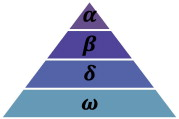
\includegraphics[width=0.4\textwidth]{assets/img/Grey_wolf_social_hierarchy.jpg}
        \caption[Soziale Hierarchie bei Grauwölfen]{Soziale Hierarchie bei Grauwölfen \cite{MIRJALILI201446}}
        \label{gwo_hierarchy}
    \end{center}
\end{figure}

\subsection{Jagdverhalten}
Neben dem Sozialverhalten ist das Jagdverhalten der Grauwölfe von besonderem Interesse. Dieses teilt sich nach \cite[vgl. Mirjalili 2014, S.5]{MIRJALILI201446} in folgende Phasen: 
\begin{itemize}
    \item Suchen, Jagen und Erreichen der Beute
    \item Verfolgen, Einkreisen und Beunruhigen der Beute, bis sie stehen bleibt
    \item Angreifen der Beute 
\end{itemize}
% \begin{figure}[ht]
%     \begin{center}
%         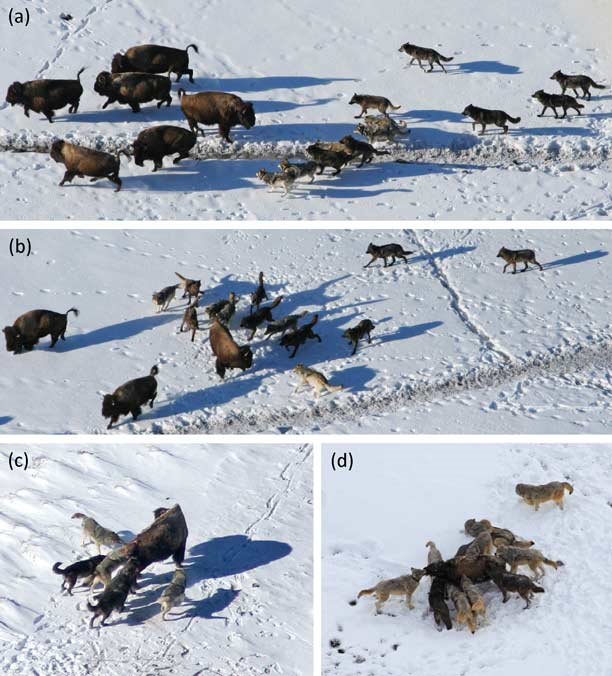
\includegraphics[width=0.9\textwidth]{assets/img/wolf-hunt-study_plos_612x676.png}
%         \caption[Jagdverhalten bei Grauwölfen]{Jagdverhalten bei Grauwölfen \cite{yellowstoneparkWolfhunt}}
%         \label{gwo_hunt}
%     \end{center}
% \end{figure}
% Diese Phasen sind in \autoref{gwo_hunt} dargestellt.\\
Der Algorithmus 'Grey Wolf Optimization' stützt sich auf die mathematische Umsetzung des Jagdverhaltens und des Sozialverhaltens von Grauwölfen.
